\documentclass{article}
\usepackage[utf8]{inputenc}
\usepackage[T2A]{fontenc}
\usepackage[russian]{babel}

\usepackage{natbib}
\usepackage{graphicx}
\usepackage{amsmath}
\usepackage{xcolor}
\usepackage{amssymb}
\usepackage{graphicx}
\usepackage[paper=a4paper, margin=2cm, bottom=2cm]{geometry}
\usepackage{pythonhighlight}

\begin{document}
\begin{titlepage}


\newgeometry{margin=1cm}

\centerline{\large \bf МИНИСТЕРСТВО ОБРАЗОВАНИЯ РЕСПУБЛИКИ БЕЛАРУСЬ}
\bigskip
\bigskip
\centerline{\large \bf БЕЛОРУССКИЙ ГОСУДАРСТВЕННЫЙ УНИВЕРСИТЕТ}
\bigskip
\bigskip
\centerline{\large \bf ФАКУЛЬТЕТ ПРИКЛАДНОЙ МАТЕМАТИКИ И ИНФОРМАТИКИ}
\vfill
\centerline{\Large \bf МЕТОДЫ ЧИСЛЕННОГО АНАЛИЗА}
\bigskip
\vfill

\centerline{\Large \bf Лабараторная работа №2}
\bigskip
\centerline{\Large \bf Приближение функций с помощью кубического сплайна}
\vfill

\hfill
\begin{minipage}{0.25\textwidth}
	{\large{\bf Студент \\ 2 курса 2 группы} \\
		{\it Царик Виталий \\ Александрович }}
\end{minipage}

\vfill
\hfill
\begin{minipage}{0.25\textwidth}
  {\large{\bf Преподаватель} \\
{\it Никифоров Иван \\ Васильевич}}
\end{minipage}
\vfill
\vfill
\centerline{\Large \bf Минск 2019}

\end{titlepage}

\restoregeometry

\section{Условие}
Отрезок $[a, b]$ разбить на 10, 20, 40 отрезков. На каждом отрезке приблизить функцию кубическим сплайном по узлам Чебышева. Для каждого из 3 случаев (n=10,20,40) построить график.

\section{Вариант}
\begin{equation}
\label{eq:variant}
f(x) = -\frac{1}{x} + x + x^2, x \in [1, 2]
\end{equation}

\section{Теория}

Узлы Чебышева вычисляются по формуле:
\begin{equation}
\label{eq:node}
x_k = \dfrac{a+b}{2} + \dfrac{b-a}{2} \cos{\left(\dfrac{2k+1}{2(n+1)} \pi\right)}, k = \overline{1, n} 
\end{equation} \\

\section{Графики}

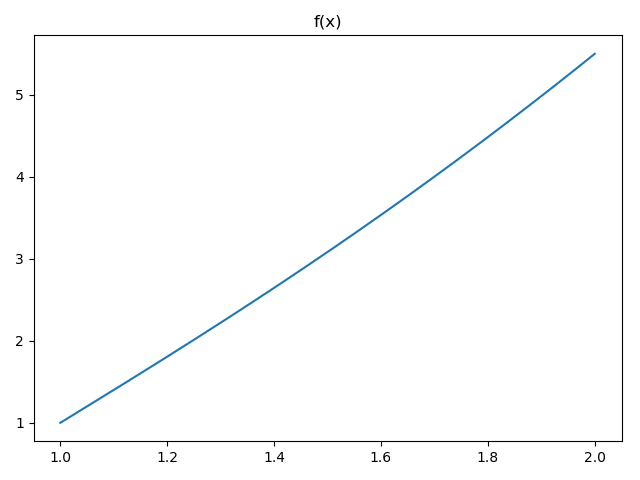
\includegraphics[scale=0.5]{f(x).png}

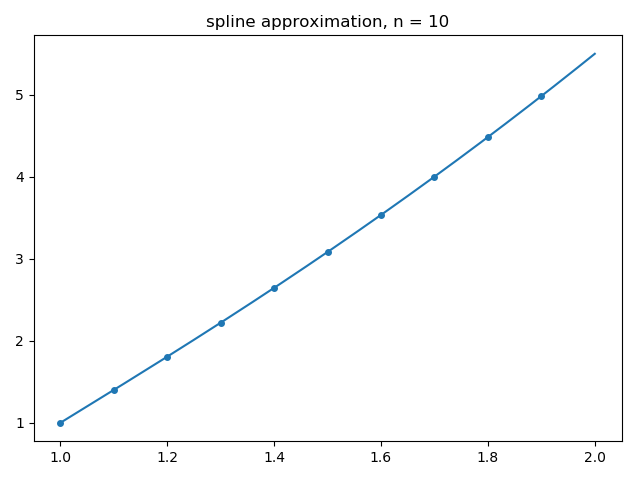
\includegraphics[scale=0.5]{10.png}

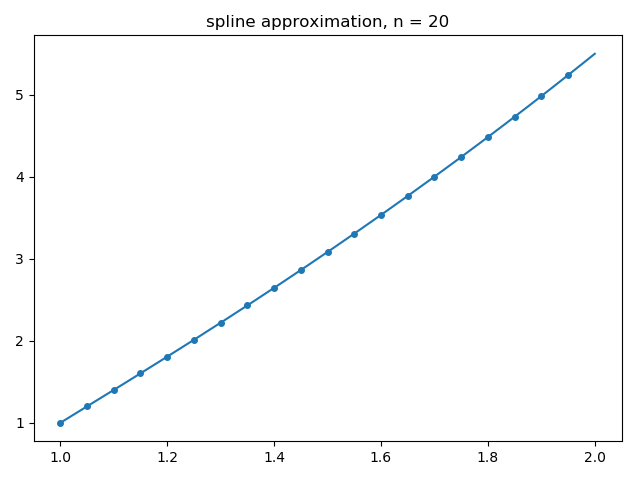
\includegraphics[scale=0.5]{20.png}

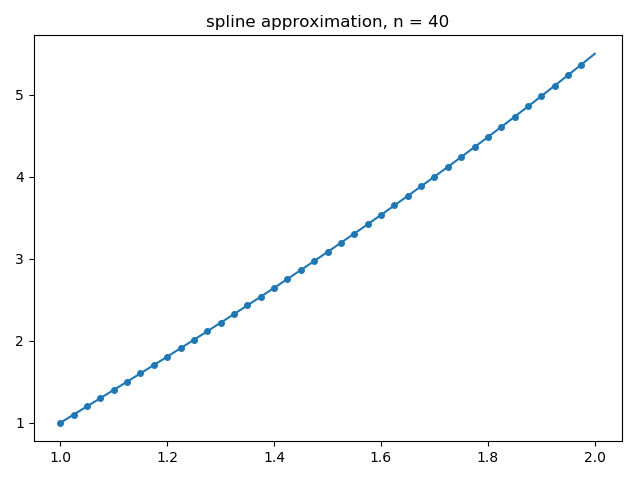
\includegraphics[scale=0.5]{40.png}

\section{Исходный код}

\begin{python}
import math
import numpy as np
import matplotlib.pyplot as plt
from scipy.interpolate import CubicSpline

n = (10, 20, 40)
A = 1
B = 2
RANK = 3
NUMBER_OF_NODES = RANK + 1


def f(x):
	return -1/x + x + x*x


def chebyshev_nodes(a, b, n):
	return np.array(
		([(a + b) / 2.0 + (b - a) / 2.0 * math.cos((2 * i + 1) / (2.0 * n + 2.0) * math.pi)
		for i in range(n)]), dtype='float')


if __name__ == '__main__':
	x = np.linspace(A, B, 10000)
	plt.plot(x, f(x))
	plt.title('f(x)')
	plt.show()

	for n_i in n:
		beg = A
		step = (B - A) / n_i
		end = beg

		x = []
		y = []
		for i in range(n_i):
		beg = end
		end += step

		nodes = chebyshev_nodes(beg, end, NUMBER_OF_NODES)
		nodes.sort()
		polynom = CubicSpline(nodes, f(nodes))

		x_i = np.linspace(beg, end, 100)
		x.extend(x_i)
		y.extend(polynom(x_i))

	plt.title('spline approximation, n = {}'.format(n_i))
	plt.plot(x, y, 'o', ls='-', ms=4, markevery=100, label='polynom')
	plt.show()

\end{python}

\section{Выводы}

Приближение с помощью кубического сплайна являются довольно точным для данной функции даже при относительно небольших значениях $n$

\end{document}